%% Standalone source of one report figure. Rebuild: pdflatex -output-directory=.. fig-01-architecture.tex
\documentclass[11pt]{standalone}
\usepackage[T1]{fontenc}
\usepackage[utf8]{inputenc}
\usepackage{lmodern}
\usepackage{microtype}
\usepackage{amsmath,amssymb}
\usepackage{xcolor}
\usepackage{tikz}
\usetikzlibrary{arrows.meta,positioning,shapes.geometric,fit,calc,backgrounds}
\usepackage{pgfplots}
\usepackage{pgfplotstable}
\pgfplotsset{compat=1.18}
\setlength{\textwidth}{472.31595pt}  %% = the report's text width, so widths given in \textwidth match
\definecolor{gmblue}{HTML}{0B3D6E}
\definecolor{gmok}{HTML}{1E7B34}
\definecolor{gmwarn}{HTML}{B35C00}
\definecolor{gmbad}{HTML}{A32020}
\definecolor{gmgrey}{HTML}{5A5F66}
\definecolor{gmlight}{HTML}{EEF3F8}
\definecolor{gmteal}{HTML}{1B7A8C}
\newcommand{\done}{\textcolor{gmok}{\textbf{Done}}}
\newcommand{\partly}{\textcolor{gmwarn}{\textbf{Partly}}}
\newcommand{\pending}{\textcolor{gmbad}{\textbf{Pending}}}
\newcommand{\pass}{\textcolor{gmok}{\textbf{PASS}}}
\newcommand{\fail}{\textcolor{gmbad}{\textbf{FAIL}}}
\newcommand{\code}[1]{\texttt{\small #1}}
\newcommand{\INR}{INR~}
\newcommand{\gbar}[5]{\fill[#5] (#1,-#3+0.32) rectangle (#2,-#3-0.32);
  \node[anchor=east,font=\scriptsize] at (-0.3,-#3) {#4};}

\tikzset{
  box/.style={draw=gmblue, rounded corners=3pt, fill=gmlight, align=center, font=\small, inner sep=5pt,
              minimum height=9mm},
  gstep/.style={draw=gmblue, rounded corners=3pt, fill=white, align=center, font=\footnotesize, inner sep=4pt,
               text width=27mm, minimum height=11mm},
  st/.style={draw=gmblue, rounded corners=6pt, fill=gmlight, font=\scriptsize\ttfamily, inner sep=3pt,
             minimum height=6mm},
  arr/.style={-{Stealth[length=2.2mm]}, thick, gmblue},
  darr/.style={-{Stealth[length=2mm]}, gmgrey, dashed},
}

\begin{document}
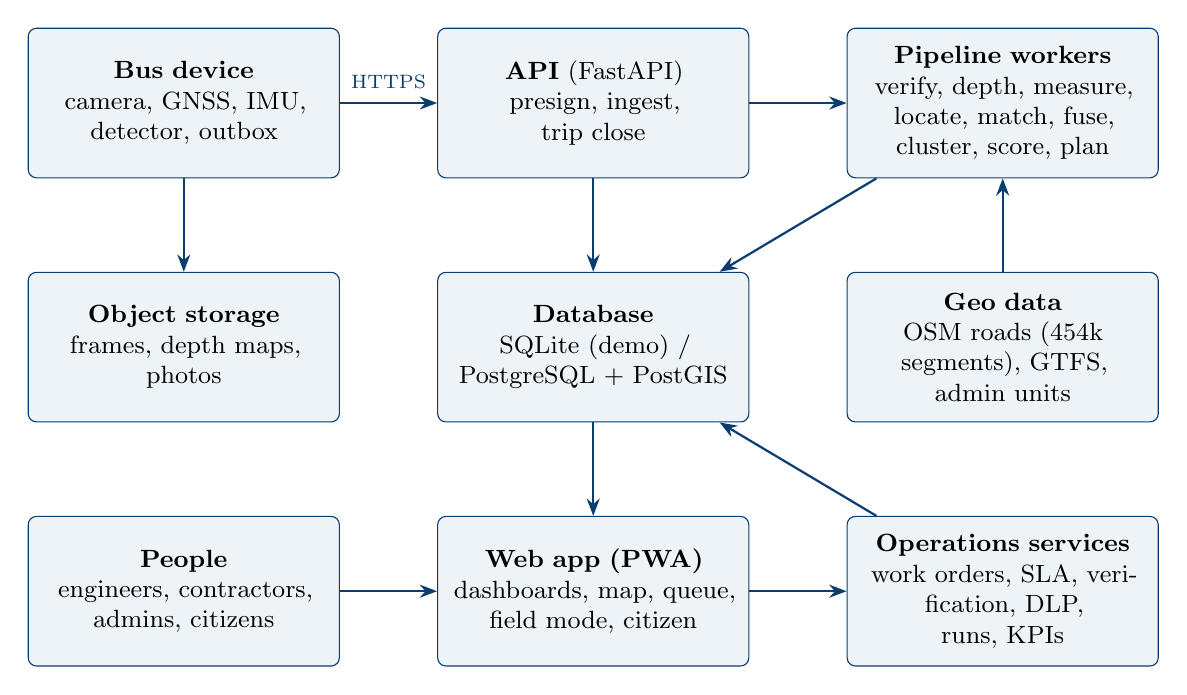
\begin{tikzpicture}[every node/.style={box, text width=36mm, minimum height=19mm}]
  \node (bus)   at (0,0)       {\textbf{Bus device}\\camera, GNSS, IMU,\\detector, outbox};
  \node (api)   at (5.2,0)     {\textbf{API} (FastAPI)\\presign, ingest,\\trip close};
  \node (pipe)  at (10.4,0)    {\textbf{Pipeline workers}\\verify, depth, measure,\\locate, match, fuse,\\cluster, score, plan};
  \node (store) at (0,-3.1)    {\textbf{Object storage}\\frames, depth maps,\\photos};
  \node (db)    at (5.2,-3.1)  {\textbf{Database}\\SQLite (demo) /\\PostgreSQL + PostGIS};
  \node (geo)   at (10.4,-3.1) {\textbf{Geo data}\\OSM roads (454k\\segments), GTFS,\\admin units};
  \node (cit)   at (0,-6.2)    {\textbf{People}\\engineers, contractors,\\admins, citizens};
  \node (web)   at (5.2,-6.2)  {\textbf{Web app (PWA)}\\dashboards, map, queue,\\field mode, citizen};
  \node (ops)   at (10.4,-6.2) {\textbf{Operations services}\\work orders, SLA, veri-\\fication, DLP, runs, KPIs};
  \draw[arr] (bus) -- node[above, draw=none, fill=none, text width=, minimum height=0pt, font=\scriptsize]{HTTPS} (api);
  \draw[arr] (api) -- (pipe);
  \draw[arr] (bus) -- (store);
  \draw[arr] (api) -- (db);
  \draw[arr] (pipe) -- (db);
  \draw[arr] (geo) -- (pipe);
  \draw[arr] (ops) -- (db);
  \draw[arr] (db) -- (web);
  \draw[arr] (cit) -- (web);
  \draw[arr] (web) -- (ops);
\end{tikzpicture}
\end{document}
